\documentclass[twoside]{book}

% Packages required by doxygen
\usepackage{fixltx2e}
\usepackage{calc}
\usepackage{doxygen}
\usepackage[export]{adjustbox} % also loads graphicx
\usepackage{graphicx}
\usepackage[utf8]{inputenc}
\usepackage{makeidx}
\usepackage{multicol}
\usepackage{multirow}
\PassOptionsToPackage{warn}{textcomp}
\usepackage{textcomp}
\usepackage[nointegrals]{wasysym}
\usepackage[table]{xcolor}

% Font selection
\usepackage[T1]{fontenc}
\usepackage[scaled=.90]{helvet}
\usepackage{courier}
\usepackage{amssymb}
\usepackage{sectsty}
\renewcommand{\familydefault}{\sfdefault}
\allsectionsfont{%
  \fontseries{bc}\selectfont%
  \color{darkgray}%
}
\renewcommand{\DoxyLabelFont}{%
  \fontseries{bc}\selectfont%
  \color{darkgray}%
}
\newcommand{\+}{\discretionary{\mbox{\scriptsize$\hookleftarrow$}}{}{}}

% Page & text layout
\usepackage{geometry}
\geometry{%
  a4paper,%
  top=2.5cm,%
  bottom=2.5cm,%
  left=2.5cm,%
  right=2.5cm%
}
\tolerance=750
\hfuzz=15pt
\hbadness=750
\setlength{\emergencystretch}{15pt}
\setlength{\parindent}{0cm}
\setlength{\parskip}{3ex plus 2ex minus 2ex}
\makeatletter
\renewcommand{\paragraph}{%
  \@startsection{paragraph}{4}{0ex}{-1.0ex}{1.0ex}{%
    \normalfont\normalsize\bfseries\SS@parafont%
  }%
}
\renewcommand{\subparagraph}{%
  \@startsection{subparagraph}{5}{0ex}{-1.0ex}{1.0ex}{%
    \normalfont\normalsize\bfseries\SS@subparafont%
  }%
}
\makeatother

% Headers & footers
\usepackage{fancyhdr}
\pagestyle{fancyplain}
\fancyhead[LE]{\fancyplain{}{\bfseries\thepage}}
\fancyhead[CE]{\fancyplain{}{}}
\fancyhead[RE]{\fancyplain{}{\bfseries\leftmark}}
\fancyhead[LO]{\fancyplain{}{\bfseries\rightmark}}
\fancyhead[CO]{\fancyplain{}{}}
\fancyhead[RO]{\fancyplain{}{\bfseries\thepage}}
\fancyfoot[LE]{\fancyplain{}{}}
\fancyfoot[CE]{\fancyplain{}{}}
\fancyfoot[RE]{\fancyplain{}{\bfseries\scriptsize Generated by Doxygen }}
\fancyfoot[LO]{\fancyplain{}{\bfseries\scriptsize Generated by Doxygen }}
\fancyfoot[CO]{\fancyplain{}{}}
\fancyfoot[RO]{\fancyplain{}{}}
\renewcommand{\footrulewidth}{0.4pt}
\renewcommand{\chaptermark}[1]{%
  \markboth{#1}{}%
}
\renewcommand{\sectionmark}[1]{%
  \markright{\thesection\ #1}%
}

% Indices & bibliography
\usepackage{natbib}
\usepackage[titles]{tocloft}
\setcounter{tocdepth}{3}
\setcounter{secnumdepth}{5}
\makeindex

% Hyperlinks (required, but should be loaded last)
\usepackage{ifpdf}
\ifpdf
  \usepackage[pdftex,pagebackref=true]{hyperref}
\else
  \usepackage[ps2pdf,pagebackref=true]{hyperref}
\fi
\hypersetup{%
  colorlinks=true,%
  linkcolor=blue,%
  citecolor=blue,%
  unicode%
}

% Custom commands
\newcommand{\clearemptydoublepage}{%
  \newpage{\pagestyle{empty}\cleardoublepage}%
}

\usepackage{caption}
\captionsetup{labelsep=space,justification=centering,font={bf},singlelinecheck=off,skip=4pt,position=top}

%===== C O N T E N T S =====

\begin{document}

% Titlepage & ToC
\hypersetup{pageanchor=false,
             bookmarksnumbered=true,
             pdfencoding=unicode
            }
\pagenumbering{roman}
\begin{titlepage}
\vspace*{7cm}
\begin{center}%
{\Large My Project }\\
\vspace*{1cm}
{\large Generated by Doxygen 1.8.11}\\
\end{center}
\end{titlepage}
\clearemptydoublepage
\tableofcontents
\clearemptydoublepage
\pagenumbering{arabic}
\hypersetup{pageanchor=true}

%--- Begin generated contents ---
\chapter{Class Index}
\section{Class List}
Here are the classes, structs, unions and interfaces with brief descriptions\+:\begin{DoxyCompactList}
\item\contentsline{section}{\hyperlink{structcollision}{collision} }{\pageref{structcollision}}{}
\item\contentsline{section}{\hyperlink{structentity}{entity} }{\pageref{structentity}}{}
\item\contentsline{section}{\hyperlink{structimage}{image} }{\pageref{structimage}}{}
\item\contentsline{section}{\hyperlink{structinput}{input} }{\pageref{structinput}}{}
\item\contentsline{section}{\hyperlink{structmap}{map} }{\pageref{structmap}}{}
\item\contentsline{section}{\hyperlink{structpersonnage}{personnage} \\*Struct for the personnage }{\pageref{structpersonnage}}{}
\item\contentsline{section}{\hyperlink{structtext}{text} }{\pageref{structtext}}{}
\item\contentsline{section}{\hyperlink{structthe}{the} \\*Struct for the entity }{\pageref{structthe}}{}
\item\contentsline{section}{\hyperlink{structtime}{time} }{\pageref{structtime}}{}
\end{DoxyCompactList}

\chapter{File Index}
\section{File List}
Here is a list of all documented files with brief descriptions\+:\begin{DoxyCompactList}
\item\contentsline{section}{\hyperlink{entity_8c}{entity.\+c} }{\pageref{entity_8c}}{}
\item\contentsline{section}{{\bfseries entity.\+h} }{\pageref{entity_8h}}{}
\item\contentsline{section}{\hyperlink{main_8c}{main.\+c} \\*Exécution de programme }{\pageref{main_8c}}{}
\item\contentsline{section}{\hyperlink{map_8c}{map.\+c} }{\pageref{map_8c}}{}
\item\contentsline{section}{{\bfseries map.\+h} }{\pageref{map_8h}}{}
\item\contentsline{section}{{\bfseries utilitaire.\+h} }{\pageref{utilitaire_8h}}{}
\end{DoxyCompactList}

\chapter{Class Documentation}
\hypertarget{structcollision}{}\section{collision Struct Reference}
\label{structcollision}\index{collision@{collision}}
\subsection*{Public Attributes}
\begin{DoxyCompactItemize}
\item 
int {\bfseries colbackgenigme}\hypertarget{structcollision_abcf86bca0068fca534f11c600c941da0}{}\label{structcollision_abcf86bca0068fca534f11c600c941da0}

\item 
int {\bfseries colcoin}\hypertarget{structcollision_a103941a41d31cbdb5a58c24fc75089a4}{}\label{structcollision_a103941a41d31cbdb5a58c24fc75089a4}

\item 
int {\bfseries colenmie}\hypertarget{structcollision_a71198421cdcfa728868a19e9e24507dc}{}\label{structcollision_a71198421cdcfa728868a19e9e24507dc}

\item 
int {\bfseries colenigme}\hypertarget{structcollision_a1ac28c83a10d8349661c5924338d5aa4}{}\label{structcollision_a1ac28c83a10d8349661c5924338d5aa4}

\item 
int {\bfseries colbackgtrou}\hypertarget{structcollision_abb7c93a7aed306b754319095b1dae1f7}{}\label{structcollision_abb7c93a7aed306b754319095b1dae1f7}

\end{DoxyCompactItemize}


The documentation for this struct was generated from the following file\+:\begin{DoxyCompactItemize}
\item 
utilitaire.\+h\end{DoxyCompactItemize}

\hypertarget{structentity}{}\section{entity Struct Reference}
\label{structentity}\index{entity@{entity}}
\subsection*{Public Attributes}
\begin{DoxyCompactItemize}
\item 
S\+D\+L\+\_\+\+Surface $\ast$ \hyperlink{structentity_a1d532bf2d860422dbcdbf5a3d53bec2a}{entity}
\item 
S\+D\+L\+\_\+\+Rect \hyperlink{structentity_afad5429807d112e50d95031d2a7317ca}{pos\+\_\+entity}
\item 
S\+D\+L\+\_\+\+Rect \hyperlink{structentity_a854a764985b0f1ae5969d3d31534dafc}{anim\+\_\+entity} \mbox{[}70\mbox{]}
\item 
int {\bfseries frame\+\_\+entity}\hypertarget{structentity_a60fd1d07d2b5e6c5e02d3a10d51cec8a}{}\label{structentity_a60fd1d07d2b5e6c5e02d3a10d51cec8a}

\item 
int {\bfseries direction}\hypertarget{structentity_a643c70cbdbf48c0e06d66c2d20ada874}{}\label{structentity_a643c70cbdbf48c0e06d66c2d20ada874}

\item 
int {\bfseries col}\hypertarget{structentity_a5e6a4bc4a8cbd87a5003ac338a832fa7}{}\label{structentity_a5e6a4bc4a8cbd87a5003ac338a832fa7}

\item 
int {\bfseries type}\hypertarget{structentity_afb415e14577c5fc356ae19ad90aa36f3}{}\label{structentity_afb415e14577c5fc356ae19ad90aa36f3}

\item 
int {\bfseries max\+\_\+up}\hypertarget{structentity_ad35af5a0d54177d169f799bd4cebf767}{}\label{structentity_ad35af5a0d54177d169f799bd4cebf767}

\item 
int {\bfseries max\+\_\+down}\hypertarget{structentity_a82abfb3de23d8fb9ddc6ce8354050113}{}\label{structentity_a82abfb3de23d8fb9ddc6ce8354050113}

\item 
int {\bfseries show}\hypertarget{structentity_a3eda708ba5febdc2d10698d31131fb5d}{}\label{structentity_a3eda708ba5febdc2d10698d31131fb5d}

\end{DoxyCompactItemize}


\subsection{Member Data Documentation}
\index{entity@{entity}!anim\+\_\+entity@{anim\+\_\+entity}}
\index{anim\+\_\+entity@{anim\+\_\+entity}!entity@{entity}}
\subsubsection[{\texorpdfstring{anim\+\_\+entity}{anim_entity}}]{\setlength{\rightskip}{0pt plus 5cm}S\+D\+L\+\_\+\+Rect entity\+::anim\+\_\+entity\mbox{[}70\mbox{]}}\hypertarget{structentity_a854a764985b0f1ae5969d3d31534dafc}{}\label{structentity_a854a764985b0f1ae5969d3d31534dafc}
Rectangle \index{entity@{entity}!entity@{entity}}
\index{entity@{entity}!entity@{entity}}
\subsubsection[{\texorpdfstring{entity}{entity}}]{\setlength{\rightskip}{0pt plus 5cm}S\+D\+L\+\_\+\+Surface$\ast$ entity\+::entity}\hypertarget{structentity_a1d532bf2d860422dbcdbf5a3d53bec2a}{}\label{structentity_a1d532bf2d860422dbcdbf5a3d53bec2a}
Surface. \index{entity@{entity}!pos\+\_\+entity@{pos\+\_\+entity}}
\index{pos\+\_\+entity@{pos\+\_\+entity}!entity@{entity}}
\subsubsection[{\texorpdfstring{pos\+\_\+entity}{pos_entity}}]{\setlength{\rightskip}{0pt plus 5cm}S\+D\+L\+\_\+\+Rect entity\+::pos\+\_\+entity}\hypertarget{structentity_afad5429807d112e50d95031d2a7317ca}{}\label{structentity_afad5429807d112e50d95031d2a7317ca}
Rectangle 

The documentation for this struct was generated from the following file\+:\begin{DoxyCompactItemize}
\item 
entity.\+h\end{DoxyCompactItemize}

\hypertarget{structimage}{}\section{image Struct Reference}
\label{structimage}\index{image@{image}}
\subsection*{Public Attributes}
\begin{DoxyCompactItemize}
\item 
S\+D\+L\+\_\+\+Surface $\ast$ {\bfseries image}\hypertarget{structimage_a68c71e2eca756ac70ef1b8a2339a5e3f}{}\label{structimage_a68c71e2eca756ac70ef1b8a2339a5e3f}

\item 
S\+D\+L\+\_\+\+Rect {\bfseries posimage}\hypertarget{structimage_a3a1da83b39faccddb0cd937844ba9e0b}{}\label{structimage_a3a1da83b39faccddb0cd937844ba9e0b}

\end{DoxyCompactItemize}


The documentation for this struct was generated from the following file\+:\begin{DoxyCompactItemize}
\item 
utilitaire.\+h\end{DoxyCompactItemize}

\hypertarget{structinput}{}\section{input Struct Reference}
\label{structinput}\index{input@{input}}
\subsection*{Public Attributes}
\begin{DoxyCompactItemize}
\item 
int {\bfseries clavier} \mbox{[}322\mbox{]}\hypertarget{structinput_a16310d492ad445ab28f8967aa370cbdc}{}\label{structinput_a16310d492ad445ab28f8967aa370cbdc}

\item 
int {\bfseries souris} \mbox{[}3\mbox{]}\hypertarget{structinput_a8c22f8ed0c0b5b39742ed43aaffad224}{}\label{structinput_a8c22f8ed0c0b5b39742ed43aaffad224}

\end{DoxyCompactItemize}


The documentation for this struct was generated from the following file\+:\begin{DoxyCompactItemize}
\item 
utilitaire.\+h\end{DoxyCompactItemize}

\hypertarget{structmap}{}\section{map Struct Reference}
\label{structmap}\index{map@{map}}
\subsection*{Public Attributes}
\begin{DoxyCompactItemize}
\item 
S\+D\+L\+\_\+\+Surface $\ast$ \hyperlink{structmap_a32daf60eeab6910e405dc049350b1e9c}{map}
\item 
S\+D\+L\+\_\+\+Rect \hyperlink{structmap_a892e2b0bcb168e8a85bd000b1bda0611}{pos\+\_\+map}
\item 
S\+D\+L\+\_\+\+Surface $\ast$ {\bfseries mini\+\_\+entity}\hypertarget{structmap_af5cb6ef5d8d995a8441e8bfc8fd5c862}{}\label{structmap_af5cb6ef5d8d995a8441e8bfc8fd5c862}

\item 
S\+D\+L\+\_\+\+Rect {\bfseries entity\+\_\+pos\+\_\+map}\hypertarget{structmap_acc2166f6c1dcbc1d8bb9a389b5bfb578}{}\label{structmap_acc2166f6c1dcbc1d8bb9a389b5bfb578}

\item 
S\+D\+L\+\_\+\+Surface $\ast$ {\bfseries mini\+\_\+perso}\hypertarget{structmap_ad5f6a0f500cd8ef220867a7821223897}{}\label{structmap_ad5f6a0f500cd8ef220867a7821223897}

\item 
S\+D\+L\+\_\+\+Rect {\bfseries perso\+\_\+pos\+\_\+map}\hypertarget{structmap_a214838f7c4a02b8148a39fbcb013282a}{}\label{structmap_a214838f7c4a02b8148a39fbcb013282a}

\end{DoxyCompactItemize}


\subsection{Member Data Documentation}
\index{map@{map}!map@{map}}
\index{map@{map}!map@{map}}
\subsubsection[{\texorpdfstring{map}{map}}]{\setlength{\rightskip}{0pt plus 5cm}S\+D\+L\+\_\+\+Surface$\ast$ map\+::map}\hypertarget{structmap_a32daf60eeab6910e405dc049350b1e9c}{}\label{structmap_a32daf60eeab6910e405dc049350b1e9c}
Surface. \index{map@{map}!pos\+\_\+map@{pos\+\_\+map}}
\index{pos\+\_\+map@{pos\+\_\+map}!map@{map}}
\subsubsection[{\texorpdfstring{pos\+\_\+map}{pos_map}}]{\setlength{\rightskip}{0pt plus 5cm}S\+D\+L\+\_\+\+Rect map\+::pos\+\_\+map}\hypertarget{structmap_a892e2b0bcb168e8a85bd000b1bda0611}{}\label{structmap_a892e2b0bcb168e8a85bd000b1bda0611}
Rectangle 

The documentation for this struct was generated from the following file\+:\begin{DoxyCompactItemize}
\item 
map.\+h\end{DoxyCompactItemize}

\hypertarget{structpersonnage}{}\section{personnage Struct Reference}
\label{structpersonnage}\index{personnage@{personnage}}


struct for the personnage  




{\ttfamily \#include $<$entity.\+h$>$}

\subsection*{Public Attributes}
\begin{DoxyCompactItemize}
\item 
S\+D\+L\+\_\+\+Surface $\ast$ \hyperlink{structpersonnage_a38531a8ef1c44bf0892c67e4c4b7f063}{perso}
\item 
S\+D\+L\+\_\+\+Rect \hyperlink{structpersonnage_ad280a2f59832f0487ef5ef3c0db45a7d}{perso\+\_\+pos}
\end{DoxyCompactItemize}


\subsection{Detailed Description}
struct for the personnage 

\subsection{Member Data Documentation}
\index{personnage@{personnage}!perso@{perso}}
\index{perso@{perso}!personnage@{personnage}}
\subsubsection[{\texorpdfstring{perso}{perso}}]{\setlength{\rightskip}{0pt plus 5cm}S\+D\+L\+\_\+\+Surface$\ast$ personnage\+::perso}\hypertarget{structpersonnage_a38531a8ef1c44bf0892c67e4c4b7f063}{}\label{structpersonnage_a38531a8ef1c44bf0892c67e4c4b7f063}
Surface. \index{personnage@{personnage}!perso\+\_\+pos@{perso\+\_\+pos}}
\index{perso\+\_\+pos@{perso\+\_\+pos}!personnage@{personnage}}
\subsubsection[{\texorpdfstring{perso\+\_\+pos}{perso_pos}}]{\setlength{\rightskip}{0pt plus 5cm}S\+D\+L\+\_\+\+Rect personnage\+::perso\+\_\+pos}\hypertarget{structpersonnage_ad280a2f59832f0487ef5ef3c0db45a7d}{}\label{structpersonnage_ad280a2f59832f0487ef5ef3c0db45a7d}
Rectangle 

The documentation for this struct was generated from the following file\+:\begin{DoxyCompactItemize}
\item 
entity.\+h\end{DoxyCompactItemize}

\hypertarget{structtext}{}\section{text Struct Reference}
\label{structtext}\index{text@{text}}
\subsection*{Public Attributes}
\begin{DoxyCompactItemize}
\item 
S\+D\+L\+\_\+\+Surface $\ast$ {\bfseries text\+Surface}\hypertarget{structtext_a1a9992f493ebd8946dc5a736d65e8213}{}\label{structtext_a1a9992f493ebd8946dc5a736d65e8213}

\item 
S\+D\+L\+\_\+\+Rect {\bfseries position\+Text}\hypertarget{structtext_a01cc24369eccbe9ccb68af9a748315d3}{}\label{structtext_a01cc24369eccbe9ccb68af9a748315d3}

\item 
char {\bfseries txt} \mbox{[}20\mbox{]}\hypertarget{structtext_afd7610607c0ade6ed450f86e275ddce5}{}\label{structtext_afd7610607c0ade6ed450f86e275ddce5}

\item 
S\+D\+L\+\_\+\+Color {\bfseries couleur\+Txt}\hypertarget{structtext_a0f3134d4dbc64c9b28fa625fb627f9c5}{}\label{structtext_a0f3134d4dbc64c9b28fa625fb627f9c5}

\item 
T\+T\+F\+\_\+\+Font $\ast$ {\bfseries police}\hypertarget{structtext_aec9ba02a1c093b1db8aa0f16ac092459}{}\label{structtext_aec9ba02a1c093b1db8aa0f16ac092459}

\end{DoxyCompactItemize}


The documentation for this struct was generated from the following file\+:\begin{DoxyCompactItemize}
\item 
utilitaire.\+h\end{DoxyCompactItemize}

\hypertarget{structthe}{}\section{the Struct Reference}
\label{structthe}\index{the@{the}}


struct for the entity  




\subsection{Detailed Description}
struct for the entity 

struct for the map 

The documentation for this struct was generated from the following file\+:\begin{DoxyCompactItemize}
\item 
entity.\+h\end{DoxyCompactItemize}

\hypertarget{structtime}{}\section{time Struct Reference}
\label{structtime}\index{time@{time}}


Collaboration diagram for time\+:\nopagebreak
\begin{figure}[H]
\begin{center}
\leavevmode
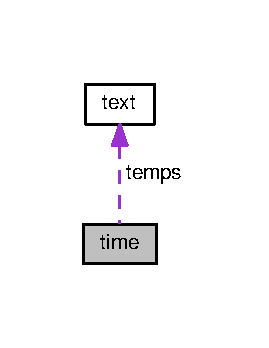
\includegraphics[width=129pt]{structtime__coll__graph}
\end{center}
\end{figure}
\subsection*{Public Attributes}
\begin{DoxyCompactItemize}
\item 
int {\bfseries tempsdebut}\hypertarget{structtime_a631b29da38929a12fb4997cb6c77ca65}{}\label{structtime_a631b29da38929a12fb4997cb6c77ca65}

\item 
int {\bfseries mm}\hypertarget{structtime_ae3e68d8be9d3f14dec119d67b848fc47}{}\label{structtime_ae3e68d8be9d3f14dec119d67b848fc47}

\item 
int {\bfseries ss}\hypertarget{structtime_a9d94f0d593508ac616752cbe36601004}{}\label{structtime_a9d94f0d593508ac616752cbe36601004}

\item 
\hyperlink{structtext}{Text} {\bfseries temps}\hypertarget{structtime_a664308034ded61bae3412c574ad3305c}{}\label{structtime_a664308034ded61bae3412c574ad3305c}

\end{DoxyCompactItemize}


The documentation for this struct was generated from the following file\+:\begin{DoxyCompactItemize}
\item 
utilitaire.\+h\end{DoxyCompactItemize}

\chapter{File Documentation}
\hypertarget{entity_8c}{}\section{entity.\+c File Reference}
\label{entity_8c}\index{entity.\+c@{entity.\+c}}
{\ttfamily \#include \char`\"{}entity.\+h\char`\"{}}\\*
Include dependency graph for entity.\+c\+:\nopagebreak
\begin{figure}[H]
\begin{center}
\leavevmode
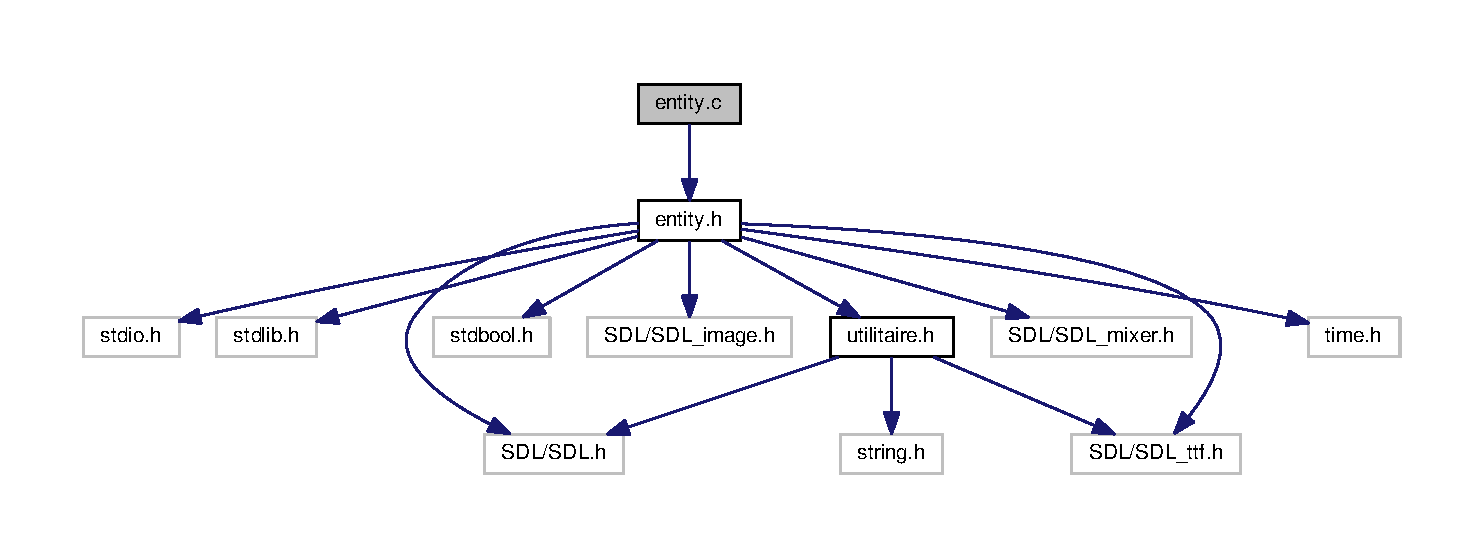
\includegraphics[width=350pt]{entity_8c__incl}
\end{center}
\end{figure}
\subsection*{Functions}
\begin{DoxyCompactItemize}
\item 
void {\bfseries init\+\_\+tab\+\_\+anim\+\_\+entity} (S\+D\+L\+\_\+\+Rect $\ast$clip, \hyperlink{structentity}{entity} $\ast$e)\hypertarget{entity_8c_ad3e342e83d35251b90b1c9e4225e2ff2}{}\label{entity_8c_ad3e342e83d35251b90b1c9e4225e2ff2}

\item 
void \hyperlink{entity_8c_a4ccd350b3198bed521c69a2498ecbc67}{initialiser\+\_\+entity} (\hyperlink{structentity}{entity} $\ast$e, int t)
\begin{DoxyCompactList}\small\item\em To initialize the entity e . \end{DoxyCompactList}\item 
void \hyperlink{entity_8c_af0abb6172652186e8763e3ceaae90729}{afficher\+\_\+entity} (\hyperlink{structentity}{entity} $\ast$e, S\+D\+L\+\_\+\+Surface $\ast$screen)
\begin{DoxyCompactList}\small\item\em To show the entity e . \end{DoxyCompactList}\item 
void \hyperlink{entity_8c_a6a59c380525a58504970c106321599d2}{mvt\+\_\+entity} (\hyperlink{structentity}{entity} $\ast$e, \hyperlink{structpersonnage}{personnage} $\ast$p)
\begin{DoxyCompactList}\small\item\em for the random movement of the secondary entity and the automation ennemi . \end{DoxyCompactList}\item 
void \hyperlink{entity_8c_a7a0c32e4b866aa8b654cf37de8a5090b}{anim} (\hyperlink{structentity}{entity} $\ast$e)
\begin{DoxyCompactList}\small\item\em for the animation the secondary entity . \end{DoxyCompactList}\item 
void \hyperlink{entity_8c_a669bdf00d6412194de61ae2bde2aa833}{update\+\_\+entity} (\hyperlink{structentity}{entity} $\ast$e, \hyperlink{structpersonnage}{personnage} $\ast$p)
\begin{DoxyCompactList}\small\item\em for the integration of two functions (anim,mouv) . \end{DoxyCompactList}\item 
void \hyperlink{entity_8c_af78186ba488162ac2cf554d640b429b2}{rand\+\_\+min\+\_\+max} (\hyperlink{structentity}{entity} $\ast$e)
\begin{DoxyCompactList}\small\item\em to change the maxi down and the maxi up randomly . \end{DoxyCompactList}\item 
\hyperlink{structinput}{input} {\bfseries getinput} (int $\ast$done, \hyperlink{structinput}{input} in)\hypertarget{entity_8c_a7214aad146b64791f5b5861d448ef61a}{}\label{entity_8c_a7214aad146b64791f5b5861d448ef61a}

\item 
void \hyperlink{entity_8c_ab76e735545868fc99b5b91849eea7d7a}{initialiser\+\_\+perso} (\hyperlink{structpersonnage}{personnage} $\ast$p)
\begin{DoxyCompactList}\small\item\em To initialize the personnage p . \end{DoxyCompactList}\item 
void \hyperlink{entity_8c_a43181619fa488bdbf458203b3a0a51c5}{afficher\+\_\+perso} (\hyperlink{structpersonnage}{personnage} $\ast$p, S\+D\+L\+\_\+\+Surface $\ast$screen)
\begin{DoxyCompactList}\small\item\em To show the personnage p . \end{DoxyCompactList}\item 
int \hyperlink{entity_8c_a49f4932b04d7655277cd407f47b7e8a1}{detect\+\_\+collision} (\hyperlink{structpersonnage}{personnage} $\ast$p, \hyperlink{structentity}{entity} $\ast$e)
\begin{DoxyCompactList}\small\item\em for the detection of a collision bounding box . \end{DoxyCompactList}\item 
int \hyperlink{entity_8c_af8b5bea828d1c0c6abffbccc337ca825}{gestion} (\hyperlink{structentity}{entity} $\ast$e)
\begin{DoxyCompactList}\small\item\em if the type of the entity is good so it will disappear in case of collision . \end{DoxyCompactList}\end{DoxyCompactItemize}
\subsection*{Variables}
\begin{DoxyCompactItemize}
\item 
int {\bfseries nb\+\_\+frame} =12\hypertarget{entity_8c_a101ab30085902e1146574a0b932fee88}{}\label{entity_8c_a101ab30085902e1146574a0b932fee88}

\item 
int {\bfseries entity\+\_\+h} =195\hypertarget{entity_8c_a8b4053c4e63d58f4018864ac683c1d5e}{}\label{entity_8c_a8b4053c4e63d58f4018864ac683c1d5e}

\item 
int {\bfseries entity\+\_\+w} =135\hypertarget{entity_8c_aff5be824c6d2567eaa775c234b0fe452}{}\label{entity_8c_aff5be824c6d2567eaa775c234b0fe452}

\item 
int {\bfseries entity\+\_\+y} =0\hypertarget{entity_8c_ac36f9a0f58bf874396ec691c59cb7eb8}{}\label{entity_8c_ac36f9a0f58bf874396ec691c59cb7eb8}

\item 
int {\bfseries entity\+\_\+x} =0\hypertarget{entity_8c_ac2ed4cd2f396112c19501c74cd093dce}{}\label{entity_8c_ac2ed4cd2f396112c19501c74cd093dce}

\item 
int {\bfseries ennemie\+\_\+h} =135\hypertarget{entity_8c_abe44642926a3738d3607f3c8ce890b34}{}\label{entity_8c_abe44642926a3738d3607f3c8ce890b34}

\item 
int {\bfseries ennemie\+\_\+w} =129\hypertarget{entity_8c_aea098e70a00577ede95d26d16a1b6d72}{}\label{entity_8c_aea098e70a00577ede95d26d16a1b6d72}

\item 
int {\bfseries ennemie\+\_\+y} =1\hypertarget{entity_8c_a6048bde8994dfe0d1aa7e8c053c2fc07}{}\label{entity_8c_a6048bde8994dfe0d1aa7e8c053c2fc07}

\item 
int {\bfseries ennemie\+\_\+x} =6\hypertarget{entity_8c_a7aa4a05ced7a06cbc7767ce470684491}{}\label{entity_8c_a7aa4a05ced7a06cbc7767ce470684491}

\end{DoxyCompactItemize}


\subsection{Function Documentation}
\index{entity.\+c@{entity.\+c}!afficher\+\_\+entity@{afficher\+\_\+entity}}
\index{afficher\+\_\+entity@{afficher\+\_\+entity}!entity.\+c@{entity.\+c}}
\subsubsection[{\texorpdfstring{afficher\+\_\+entity(entity $\ast$e, S\+D\+L\+\_\+\+Surface $\ast$screen)}{afficher_entity(entity *e, SDL_Surface *screen)}}]{\setlength{\rightskip}{0pt plus 5cm}void afficher\+\_\+entity (
\begin{DoxyParamCaption}
\item[{{\bf entity} $\ast$}]{e, }
\item[{S\+D\+L\+\_\+\+Surface $\ast$}]{screen}
\end{DoxyParamCaption}
)}\hypertarget{entity_8c_af0abb6172652186e8763e3ceaae90729}{}\label{entity_8c_af0abb6172652186e8763e3ceaae90729}


To show the entity e . 


\begin{DoxyParams}{Parameters}
{\em screen} & the screen \\
\hline
{\em e} & the entity \\
\hline
\end{DoxyParams}
\begin{DoxyReturn}{Returns}
Nothing 
\end{DoxyReturn}


Here is the call graph for this function\+:\nopagebreak
\begin{figure}[H]
\begin{center}
\leavevmode
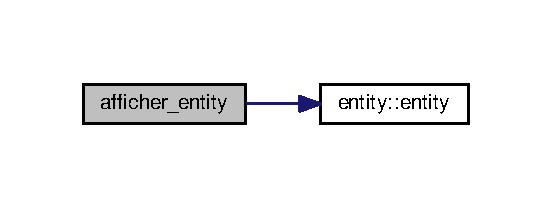
\includegraphics[width=265pt]{entity_8c_af0abb6172652186e8763e3ceaae90729_cgraph}
\end{center}
\end{figure}


\index{entity.\+c@{entity.\+c}!afficher\+\_\+perso@{afficher\+\_\+perso}}
\index{afficher\+\_\+perso@{afficher\+\_\+perso}!entity.\+c@{entity.\+c}}
\subsubsection[{\texorpdfstring{afficher\+\_\+perso(personnage $\ast$p, S\+D\+L\+\_\+\+Surface $\ast$screen)}{afficher_perso(personnage *p, SDL_Surface *screen)}}]{\setlength{\rightskip}{0pt plus 5cm}void afficher\+\_\+perso (
\begin{DoxyParamCaption}
\item[{{\bf personnage} $\ast$}]{p, }
\item[{S\+D\+L\+\_\+\+Surface $\ast$}]{screen}
\end{DoxyParamCaption}
)}\hypertarget{entity_8c_a43181619fa488bdbf458203b3a0a51c5}{}\label{entity_8c_a43181619fa488bdbf458203b3a0a51c5}


To show the personnage p . 


\begin{DoxyParams}{Parameters}
{\em screen} & the screen \\
\hline
{\em p} & the personnage \\
\hline
\end{DoxyParams}
\begin{DoxyReturn}{Returns}
Nothing 
\end{DoxyReturn}
\index{entity.\+c@{entity.\+c}!anim@{anim}}
\index{anim@{anim}!entity.\+c@{entity.\+c}}
\subsubsection[{\texorpdfstring{anim(entity $\ast$e)}{anim(entity *e)}}]{\setlength{\rightskip}{0pt plus 5cm}void anim (
\begin{DoxyParamCaption}
\item[{{\bf entity} $\ast$}]{e}
\end{DoxyParamCaption}
)}\hypertarget{entity_8c_a7a0c32e4b866aa8b654cf37de8a5090b}{}\label{entity_8c_a7a0c32e4b866aa8b654cf37de8a5090b}


for the animation the secondary entity . 


\begin{DoxyParams}{Parameters}
{\em e} & the entity \\
\hline
\end{DoxyParams}
\begin{DoxyReturn}{Returns}
Nothing 
\end{DoxyReturn}


Here is the caller graph for this function\+:\nopagebreak
\begin{figure}[H]
\begin{center}
\leavevmode
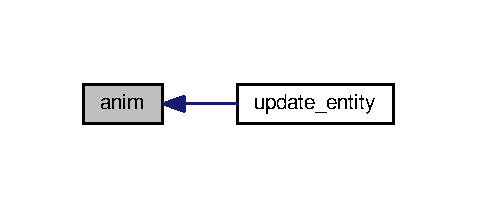
\includegraphics[width=229pt]{entity_8c_a7a0c32e4b866aa8b654cf37de8a5090b_icgraph}
\end{center}
\end{figure}


\index{entity.\+c@{entity.\+c}!detect\+\_\+collision@{detect\+\_\+collision}}
\index{detect\+\_\+collision@{detect\+\_\+collision}!entity.\+c@{entity.\+c}}
\subsubsection[{\texorpdfstring{detect\+\_\+collision(personnage $\ast$p, entity $\ast$e)}{detect_collision(personnage *p, entity *e)}}]{\setlength{\rightskip}{0pt plus 5cm}int detect\+\_\+collision (
\begin{DoxyParamCaption}
\item[{{\bf personnage} $\ast$}]{p, }
\item[{{\bf entity} $\ast$}]{e}
\end{DoxyParamCaption}
)}\hypertarget{entity_8c_a49f4932b04d7655277cd407f47b7e8a1}{}\label{entity_8c_a49f4932b04d7655277cd407f47b7e8a1}


for the detection of a collision bounding box . 


\begin{DoxyParams}{Parameters}
{\em e} & the entity \\
\hline
{\em p} & the personnage \\
\hline
\end{DoxyParams}
\begin{DoxyReturn}{Returns}
collision 
\end{DoxyReturn}
\index{entity.\+c@{entity.\+c}!gestion@{gestion}}
\index{gestion@{gestion}!entity.\+c@{entity.\+c}}
\subsubsection[{\texorpdfstring{gestion(entity $\ast$e)}{gestion(entity *e)}}]{\setlength{\rightskip}{0pt plus 5cm}int gestion (
\begin{DoxyParamCaption}
\item[{{\bf entity} $\ast$}]{e}
\end{DoxyParamCaption}
)}\hypertarget{entity_8c_af8b5bea828d1c0c6abffbccc337ca825}{}\label{entity_8c_af8b5bea828d1c0c6abffbccc337ca825}


if the type of the entity is good so it will disappear in case of collision . 


\begin{DoxyParams}{Parameters}
{\em e} & the entity \\
\hline
\end{DoxyParams}
\begin{DoxyReturn}{Returns}
0 
\end{DoxyReturn}
\index{entity.\+c@{entity.\+c}!initialiser\+\_\+entity@{initialiser\+\_\+entity}}
\index{initialiser\+\_\+entity@{initialiser\+\_\+entity}!entity.\+c@{entity.\+c}}
\subsubsection[{\texorpdfstring{initialiser\+\_\+entity(entity $\ast$e, int t)}{initialiser_entity(entity *e, int t)}}]{\setlength{\rightskip}{0pt plus 5cm}void initialiser\+\_\+entity (
\begin{DoxyParamCaption}
\item[{{\bf entity} $\ast$}]{e, }
\item[{int}]{t}
\end{DoxyParamCaption}
)}\hypertarget{entity_8c_a4ccd350b3198bed521c69a2498ecbc67}{}\label{entity_8c_a4ccd350b3198bed521c69a2498ecbc67}


To initialize the entity e . 


\begin{DoxyParams}{Parameters}
{\em e} & the entity \\
\hline
\end{DoxyParams}
\begin{DoxyReturn}{Returns}
Nothing 
\end{DoxyReturn}


Here is the call graph for this function\+:\nopagebreak
\begin{figure}[H]
\begin{center}
\leavevmode
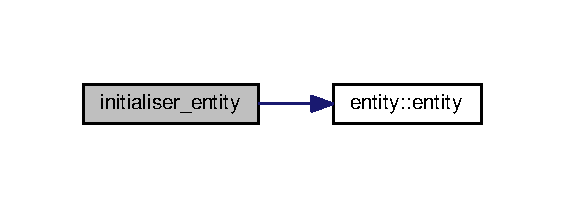
\includegraphics[width=271pt]{entity_8c_a4ccd350b3198bed521c69a2498ecbc67_cgraph}
\end{center}
\end{figure}


\index{entity.\+c@{entity.\+c}!initialiser\+\_\+perso@{initialiser\+\_\+perso}}
\index{initialiser\+\_\+perso@{initialiser\+\_\+perso}!entity.\+c@{entity.\+c}}
\subsubsection[{\texorpdfstring{initialiser\+\_\+perso(personnage $\ast$p)}{initialiser_perso(personnage *p)}}]{\setlength{\rightskip}{0pt plus 5cm}void initialiser\+\_\+perso (
\begin{DoxyParamCaption}
\item[{{\bf personnage} $\ast$}]{p}
\end{DoxyParamCaption}
)}\hypertarget{entity_8c_ab76e735545868fc99b5b91849eea7d7a}{}\label{entity_8c_ab76e735545868fc99b5b91849eea7d7a}


To initialize the personnage p . 


\begin{DoxyParams}{Parameters}
{\em p} & the personnage \\
\hline
\end{DoxyParams}
\begin{DoxyReturn}{Returns}
Nothing 
\end{DoxyReturn}
\index{entity.\+c@{entity.\+c}!mvt\+\_\+entity@{mvt\+\_\+entity}}
\index{mvt\+\_\+entity@{mvt\+\_\+entity}!entity.\+c@{entity.\+c}}
\subsubsection[{\texorpdfstring{mvt\+\_\+entity(entity $\ast$e, personnage $\ast$p)}{mvt_entity(entity *e, personnage *p)}}]{\setlength{\rightskip}{0pt plus 5cm}void mvt\+\_\+entity (
\begin{DoxyParamCaption}
\item[{{\bf entity} $\ast$}]{e, }
\item[{{\bf personnage} $\ast$}]{p}
\end{DoxyParamCaption}
)}\hypertarget{entity_8c_a6a59c380525a58504970c106321599d2}{}\label{entity_8c_a6a59c380525a58504970c106321599d2}


for the random movement of the secondary entity and the automation ennemi . 


\begin{DoxyParams}{Parameters}
{\em e} & the entity \\
\hline
{\em p} & the personnage \\
\hline
\end{DoxyParams}
\begin{DoxyReturn}{Returns}
Nothing 
\end{DoxyReturn}


Here is the call graph for this function\+:\nopagebreak
\begin{figure}[H]
\begin{center}
\leavevmode
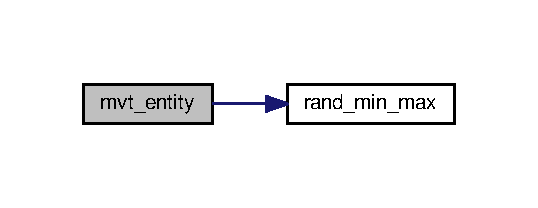
\includegraphics[width=258pt]{entity_8c_a6a59c380525a58504970c106321599d2_cgraph}
\end{center}
\end{figure}




Here is the caller graph for this function\+:\nopagebreak
\begin{figure}[H]
\begin{center}
\leavevmode
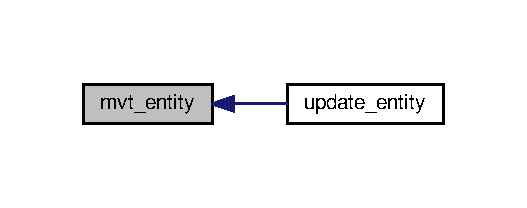
\includegraphics[width=253pt]{entity_8c_a6a59c380525a58504970c106321599d2_icgraph}
\end{center}
\end{figure}


\index{entity.\+c@{entity.\+c}!rand\+\_\+min\+\_\+max@{rand\+\_\+min\+\_\+max}}
\index{rand\+\_\+min\+\_\+max@{rand\+\_\+min\+\_\+max}!entity.\+c@{entity.\+c}}
\subsubsection[{\texorpdfstring{rand\+\_\+min\+\_\+max(entity $\ast$e)}{rand_min_max(entity *e)}}]{\setlength{\rightskip}{0pt plus 5cm}void rand\+\_\+min\+\_\+max (
\begin{DoxyParamCaption}
\item[{{\bf entity} $\ast$}]{e}
\end{DoxyParamCaption}
)}\hypertarget{entity_8c_af78186ba488162ac2cf554d640b429b2}{}\label{entity_8c_af78186ba488162ac2cf554d640b429b2}


to change the maxi down and the maxi up randomly . 


\begin{DoxyParams}{Parameters}
{\em e} & the entity \\
\hline
\end{DoxyParams}
\begin{DoxyReturn}{Returns}
Nothing 
\end{DoxyReturn}


Here is the caller graph for this function\+:\nopagebreak
\begin{figure}[H]
\begin{center}
\leavevmode
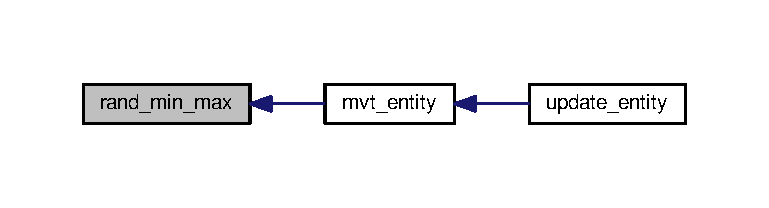
\includegraphics[width=350pt]{entity_8c_af78186ba488162ac2cf554d640b429b2_icgraph}
\end{center}
\end{figure}


\index{entity.\+c@{entity.\+c}!update\+\_\+entity@{update\+\_\+entity}}
\index{update\+\_\+entity@{update\+\_\+entity}!entity.\+c@{entity.\+c}}
\subsubsection[{\texorpdfstring{update\+\_\+entity(entity $\ast$e, personnage $\ast$p)}{update_entity(entity *e, personnage *p)}}]{\setlength{\rightskip}{0pt plus 5cm}void update\+\_\+entity (
\begin{DoxyParamCaption}
\item[{{\bf entity} $\ast$}]{e, }
\item[{{\bf personnage} $\ast$}]{p}
\end{DoxyParamCaption}
)}\hypertarget{entity_8c_a669bdf00d6412194de61ae2bde2aa833}{}\label{entity_8c_a669bdf00d6412194de61ae2bde2aa833}


for the integration of two functions (anim,mouv) . 


\begin{DoxyParams}{Parameters}
{\em e} & the entity \\
\hline
{\em p} & the personnage \\
\hline
\end{DoxyParams}
\begin{DoxyReturn}{Returns}
Nothing 
\end{DoxyReturn}


Here is the call graph for this function\+:\nopagebreak
\begin{figure}[H]
\begin{center}
\leavevmode
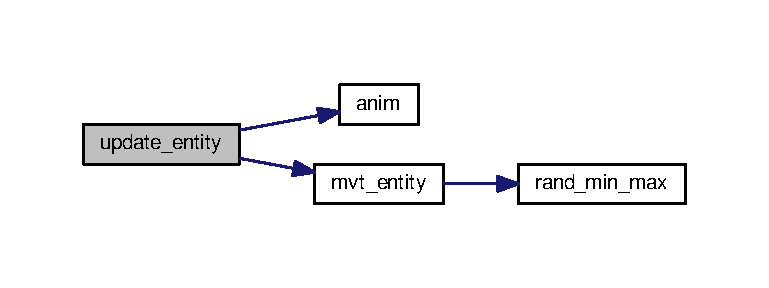
\includegraphics[width=350pt]{entity_8c_a669bdf00d6412194de61ae2bde2aa833_cgraph}
\end{center}
\end{figure}



\hypertarget{main_8c}{}\section{main.\+c File Reference}
\label{main_8c}\index{main.\+c@{main.\+c}}


exécution de programme.  


{\ttfamily \#include $<$stdio.\+h$>$}\\*
{\ttfamily \#include $<$stdlib.\+h$>$}\\*
{\ttfamily \#include $<$S\+D\+L/\+S\+D\+L.\+h$>$}\\*
{\ttfamily \#include $<$S\+D\+L/\+S\+D\+L\+\_\+image.\+h$>$}\\*
{\ttfamily \#include $<$S\+D\+L/\+S\+D\+L\+\_\+mixer.\+h$>$}\\*
{\ttfamily \#include $<$S\+D\+L/\+S\+D\+L\+\_\+ttf.\+h$>$}\\*
{\ttfamily \#include $<$time.\+h$>$}\\*
{\ttfamily \#include \char`\"{}entity.\+h\char`\"{}}\\*
{\ttfamily \#include \char`\"{}map.\+h\char`\"{}}\\*
Include dependency graph for main.\+c\+:\nopagebreak
\begin{figure}[H]
\begin{center}
\leavevmode
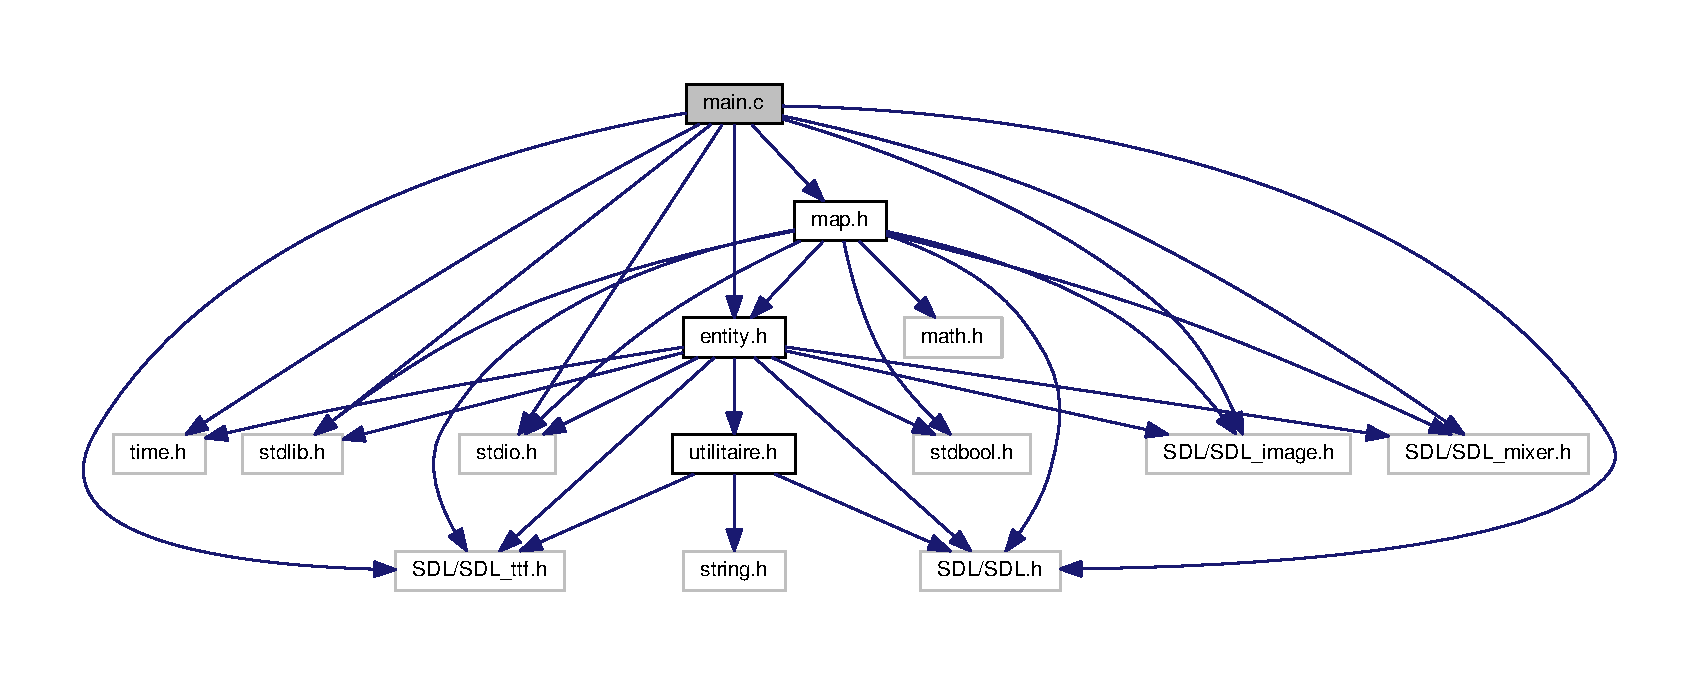
\includegraphics[width=350pt]{main_8c__incl}
\end{center}
\end{figure}
\subsection*{Functions}
\begin{DoxyCompactItemize}
\item 
int {\bfseries main} ()\hypertarget{main_8c_ae66f6b31b5ad750f1fe042a706a4e3d4}{}\label{main_8c_ae66f6b31b5ad750f1fe042a706a4e3d4}

\end{DoxyCompactItemize}


\subsection{Detailed Description}
exécution de programme. 

\begin{DoxyAuthor}{Author}
Oussama Boussetta 
\end{DoxyAuthor}
\begin{DoxyVersion}{Version}
0.\+1 
\end{DoxyVersion}
\begin{DoxyDate}{Date}
june 07, 2020
\end{DoxyDate}
exécuter le programme pour l\textquotesingle{}entitée secondaire et l\textquotesingle{}ennemi . 
\hypertarget{map_8c}{}\section{map.\+c File Reference}
\label{map_8c}\index{map.\+c@{map.\+c}}
{\ttfamily \#include \char`\"{}map.\+h\char`\"{}}\\*
Include dependency graph for map.\+c\+:\nopagebreak
\begin{figure}[H]
\begin{center}
\leavevmode
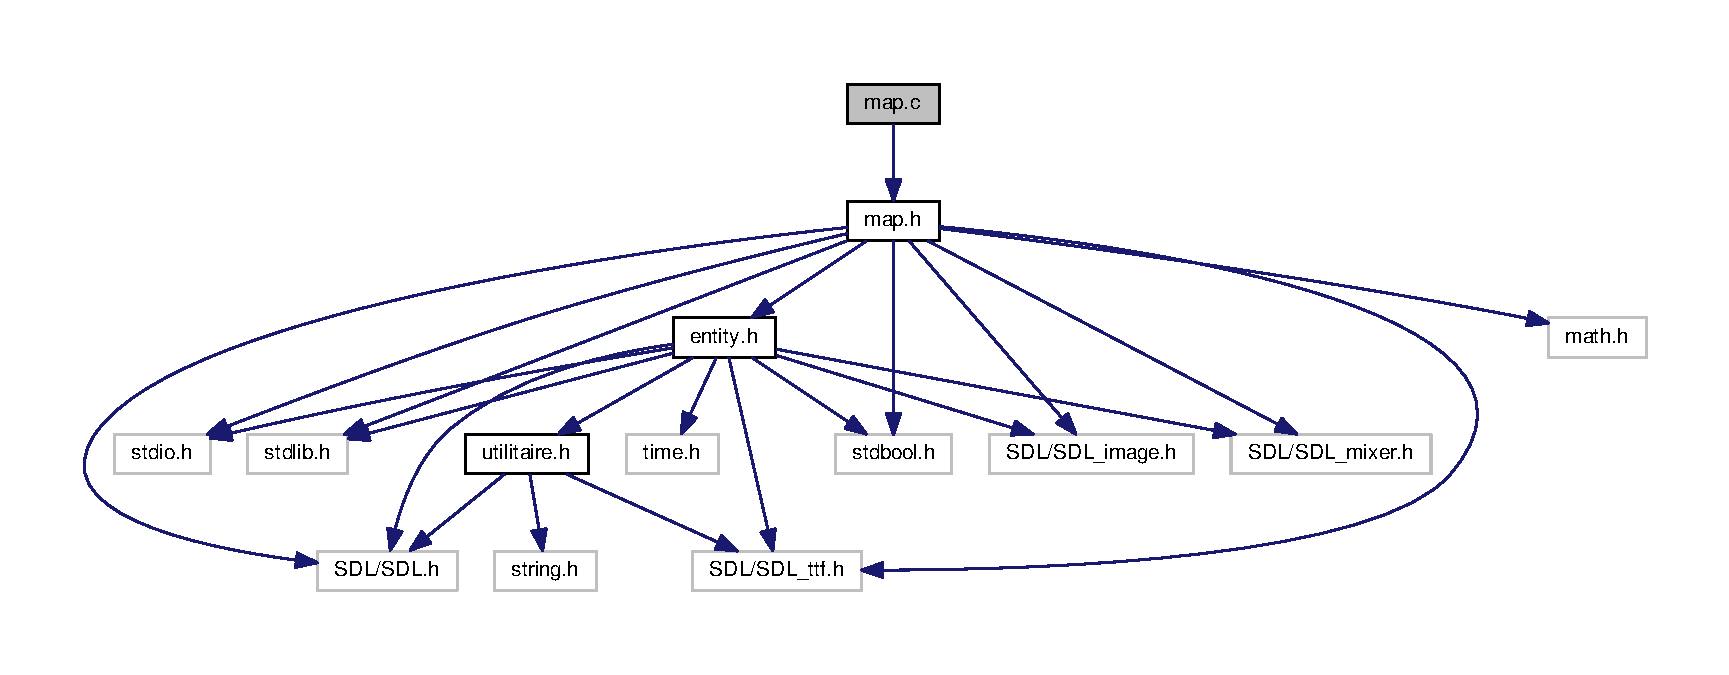
\includegraphics[width=350pt]{map_8c__incl}
\end{center}
\end{figure}
\subsection*{Functions}
\begin{DoxyCompactItemize}
\item 
void \hyperlink{map_8c_a72e7f3a5e2bcc4c7dc646cc1c04d3671}{initialiser\+\_\+map} (\hyperlink{structmap}{map} $\ast$m, S\+D\+L\+\_\+\+Surface $\ast$screen, \hyperlink{structentity}{entity} $\ast$e, \hyperlink{structpersonnage}{personnage} $\ast$p)
\begin{DoxyCompactList}\small\item\em To initialize the map m and the mini entity . \end{DoxyCompactList}\item 
void \hyperlink{map_8c_a0cc077dcdafe9f29809d29e5733876c2}{entity\+\_\+map} (\hyperlink{structmap}{map} $\ast$m, \hyperlink{structentity}{entity} $\ast$e)
\begin{DoxyCompactList}\small\item\em To initialize the postion of the mini\+\_\+entity m . \end{DoxyCompactList}\item 
void \hyperlink{map_8c_a61b189aa3bdc57b4b0d1d655060f0865}{perso\+\_\+map} (\hyperlink{structmap}{map} $\ast$m, \hyperlink{structpersonnage}{personnage} $\ast$p)
\begin{DoxyCompactList}\small\item\em To initialize the postion of the mini\+\_\+perso m . \end{DoxyCompactList}\item 
void \hyperlink{map_8c_a6f3e3fccffbe926c3c77eb06067745b1}{affiche\+\_\+map} (\hyperlink{structmap}{map} $\ast$m, S\+D\+L\+\_\+\+Surface $\ast$screen, \hyperlink{structentity}{entity} $\ast$e, \hyperlink{structpersonnage}{personnage} $\ast$p)
\begin{DoxyCompactList}\small\item\em To show the map m and the mini\+\_\+entity m and the mini\+\_\+perso p . \end{DoxyCompactList}\item 
void \hyperlink{map_8c_ae22c9d4419fe0a3287b44813affdeea0}{mise\+\_\+a\+\_\+jour\+\_\+map} (\hyperlink{structmap}{map} $\ast$m, S\+D\+L\+\_\+\+Surface $\ast$screen, \hyperlink{structpersonnage}{personnage} $\ast$p, \hyperlink{structentity}{entity} $\ast$e)
\begin{DoxyCompactList}\small\item\em for the integration of two functions (entity\+\_\+map,affiche\+\_\+map,perso\+\_\+map) . \end{DoxyCompactList}\end{DoxyCompactItemize}


\subsection{Function Documentation}
\index{map.\+c@{map.\+c}!affiche\+\_\+map@{affiche\+\_\+map}}
\index{affiche\+\_\+map@{affiche\+\_\+map}!map.\+c@{map.\+c}}
\subsubsection[{\texorpdfstring{affiche\+\_\+map(map $\ast$m, S\+D\+L\+\_\+\+Surface $\ast$screen, entity $\ast$e, personnage $\ast$p)}{affiche_map(map *m, SDL_Surface *screen, entity *e, personnage *p)}}]{\setlength{\rightskip}{0pt plus 5cm}void affiche\+\_\+map (
\begin{DoxyParamCaption}
\item[{{\bf map} $\ast$}]{m, }
\item[{S\+D\+L\+\_\+\+Surface $\ast$}]{screen, }
\item[{{\bf entity} $\ast$}]{e, }
\item[{{\bf personnage} $\ast$}]{p}
\end{DoxyParamCaption}
)}\hypertarget{map_8c_a6f3e3fccffbe926c3c77eb06067745b1}{}\label{map_8c_a6f3e3fccffbe926c3c77eb06067745b1}


To show the map m and the mini\+\_\+entity m and the mini\+\_\+perso p . 


\begin{DoxyParams}{Parameters}
{\em screen} & the screen \\
\hline
{\em m} & the map \\
\hline
{\em e} & the entity \\
\hline
{\em p} & the perso \\
\hline
\end{DoxyParams}
\begin{DoxyReturn}{Returns}
Nothing 
\end{DoxyReturn}


Here is the call graph for this function\+:\nopagebreak
\begin{figure}[H]
\begin{center}
\leavevmode
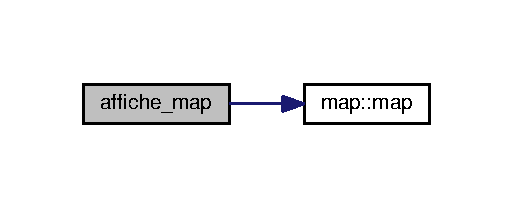
\includegraphics[width=246pt]{map_8c_a6f3e3fccffbe926c3c77eb06067745b1_cgraph}
\end{center}
\end{figure}




Here is the caller graph for this function\+:\nopagebreak
\begin{figure}[H]
\begin{center}
\leavevmode
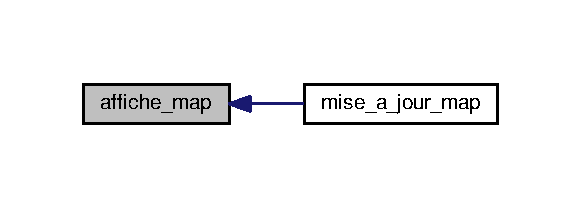
\includegraphics[width=279pt]{map_8c_a6f3e3fccffbe926c3c77eb06067745b1_icgraph}
\end{center}
\end{figure}


\index{map.\+c@{map.\+c}!entity\+\_\+map@{entity\+\_\+map}}
\index{entity\+\_\+map@{entity\+\_\+map}!map.\+c@{map.\+c}}
\subsubsection[{\texorpdfstring{entity\+\_\+map(map $\ast$m, entity $\ast$e)}{entity_map(map *m, entity *e)}}]{\setlength{\rightskip}{0pt plus 5cm}void entity\+\_\+map (
\begin{DoxyParamCaption}
\item[{{\bf map} $\ast$}]{m, }
\item[{{\bf entity} $\ast$}]{e}
\end{DoxyParamCaption}
)}\hypertarget{map_8c_a0cc077dcdafe9f29809d29e5733876c2}{}\label{map_8c_a0cc077dcdafe9f29809d29e5733876c2}


To initialize the postion of the mini\+\_\+entity m . 


\begin{DoxyParams}{Parameters}
{\em m} & the map \\
\hline
{\em e} & the entity \\
\hline
\end{DoxyParams}
\begin{DoxyReturn}{Returns}
Nothing 
\end{DoxyReturn}


Here is the caller graph for this function\+:\nopagebreak
\begin{figure}[H]
\begin{center}
\leavevmode
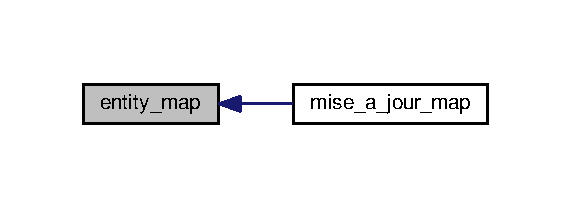
\includegraphics[width=274pt]{map_8c_a0cc077dcdafe9f29809d29e5733876c2_icgraph}
\end{center}
\end{figure}


\index{map.\+c@{map.\+c}!initialiser\+\_\+map@{initialiser\+\_\+map}}
\index{initialiser\+\_\+map@{initialiser\+\_\+map}!map.\+c@{map.\+c}}
\subsubsection[{\texorpdfstring{initialiser\+\_\+map(map $\ast$m, S\+D\+L\+\_\+\+Surface $\ast$screen, entity $\ast$e, personnage $\ast$p)}{initialiser_map(map *m, SDL_Surface *screen, entity *e, personnage *p)}}]{\setlength{\rightskip}{0pt plus 5cm}void initialiser\+\_\+map (
\begin{DoxyParamCaption}
\item[{{\bf map} $\ast$}]{m, }
\item[{S\+D\+L\+\_\+\+Surface $\ast$}]{screen, }
\item[{{\bf entity} $\ast$}]{e, }
\item[{{\bf personnage} $\ast$}]{p}
\end{DoxyParamCaption}
)}\hypertarget{map_8c_a72e7f3a5e2bcc4c7dc646cc1c04d3671}{}\label{map_8c_a72e7f3a5e2bcc4c7dc646cc1c04d3671}


To initialize the map m and the mini entity . 


\begin{DoxyParams}{Parameters}
{\em m} & map \\
\hline
{\em screen} & the screen \\
\hline
\end{DoxyParams}
\begin{DoxyReturn}{Returns}
Nothing 
\end{DoxyReturn}


Here is the call graph for this function\+:\nopagebreak
\begin{figure}[H]
\begin{center}
\leavevmode
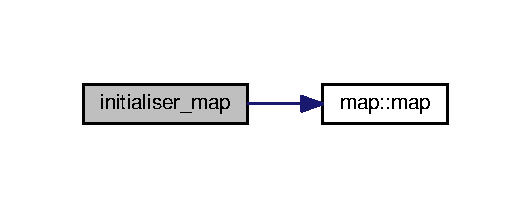
\includegraphics[width=255pt]{map_8c_a72e7f3a5e2bcc4c7dc646cc1c04d3671_cgraph}
\end{center}
\end{figure}


\index{map.\+c@{map.\+c}!mise\+\_\+a\+\_\+jour\+\_\+map@{mise\+\_\+a\+\_\+jour\+\_\+map}}
\index{mise\+\_\+a\+\_\+jour\+\_\+map@{mise\+\_\+a\+\_\+jour\+\_\+map}!map.\+c@{map.\+c}}
\subsubsection[{\texorpdfstring{mise\+\_\+a\+\_\+jour\+\_\+map(map $\ast$m, S\+D\+L\+\_\+\+Surface $\ast$screen, personnage $\ast$p, entity $\ast$e)}{mise_a_jour_map(map *m, SDL_Surface *screen, personnage *p, entity *e)}}]{\setlength{\rightskip}{0pt plus 5cm}void mise\+\_\+a\+\_\+jour\+\_\+map (
\begin{DoxyParamCaption}
\item[{{\bf map} $\ast$}]{m, }
\item[{S\+D\+L\+\_\+\+Surface $\ast$}]{screen, }
\item[{{\bf personnage} $\ast$}]{p, }
\item[{{\bf entity} $\ast$}]{e}
\end{DoxyParamCaption}
)}\hypertarget{map_8c_ae22c9d4419fe0a3287b44813affdeea0}{}\label{map_8c_ae22c9d4419fe0a3287b44813affdeea0}


for the integration of two functions (entity\+\_\+map,affiche\+\_\+map,perso\+\_\+map) . 


\begin{DoxyParams}{Parameters}
{\em m} & the map \\
\hline
{\em e} & the entity \\
\hline
{\em p} & the personnage \\
\hline
{\em screen} & the screen \\
\hline
\end{DoxyParams}
\begin{DoxyReturn}{Returns}
Nothing 
\end{DoxyReturn}


Here is the call graph for this function\+:
\nopagebreak
\begin{figure}[H]
\begin{center}
\leavevmode
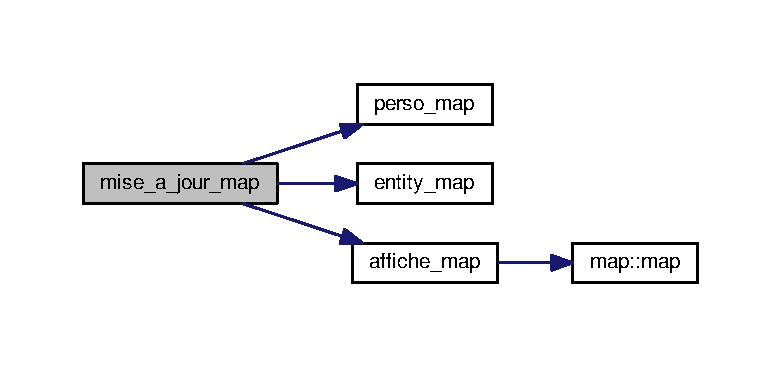
\includegraphics[width=350pt]{map_8c_ae22c9d4419fe0a3287b44813affdeea0_cgraph}
\end{center}
\end{figure}


\index{map.\+c@{map.\+c}!perso\+\_\+map@{perso\+\_\+map}}
\index{perso\+\_\+map@{perso\+\_\+map}!map.\+c@{map.\+c}}
\subsubsection[{\texorpdfstring{perso\+\_\+map(map $\ast$m, personnage $\ast$p)}{perso_map(map *m, personnage *p)}}]{\setlength{\rightskip}{0pt plus 5cm}void perso\+\_\+map (
\begin{DoxyParamCaption}
\item[{{\bf map} $\ast$}]{m, }
\item[{{\bf personnage} $\ast$}]{p}
\end{DoxyParamCaption}
)}\hypertarget{map_8c_a61b189aa3bdc57b4b0d1d655060f0865}{}\label{map_8c_a61b189aa3bdc57b4b0d1d655060f0865}


To initialize the postion of the mini\+\_\+perso m . 


\begin{DoxyParams}{Parameters}
{\em m} & the map \\
\hline
{\em p} & the perso \\
\hline
\end{DoxyParams}
\begin{DoxyReturn}{Returns}
Nothing 
\end{DoxyReturn}


Here is the caller graph for this function\+:\nopagebreak
\begin{figure}[H]
\begin{center}
\leavevmode
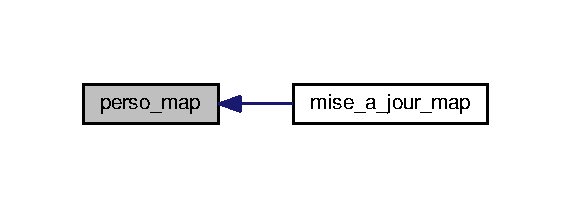
\includegraphics[width=274pt]{map_8c_a61b189aa3bdc57b4b0d1d655060f0865_icgraph}
\end{center}
\end{figure}



%--- End generated contents ---

% Index
\backmatter
\newpage
\phantomsection
\clearemptydoublepage
\addcontentsline{toc}{chapter}{Index}
\printindex

\end{document}
